\fullsys (\sys) is the abstraction of a group of batteryless intermittent sensors. \sys seeks to offer continuous sensing despite relying on ambient energy: an unpredictable and marginal power source. 
%orchestrates its nodes power cycles using a distributed approach (instead of relying on a master powerful node to coordinate coalesced nodes activities). 
%\sys seeks maximum time span of its underlying coalesced nodes through a distributed approach instead of a master node that orchestrates coalesced nodes on/off cycles. 

\subsection{Energy consumption}
%
\begin{figure}[t]
	\centering
		\begin{subfigure}{\columnwidth}
			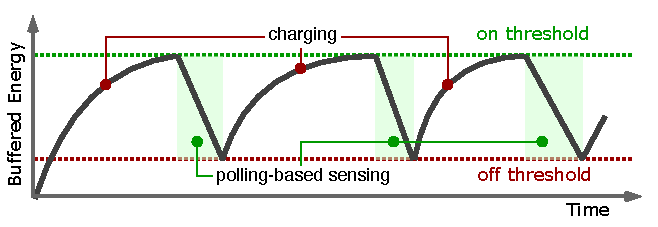
\includegraphics[width=\columnwidth]{figures/PowerCycleIntermittentSystem}
			\caption{When \sys does polling-based sensing, its energy consumption profile has, generally, two distinct rates: zero when it is charging, and a maximum when it is sensing.}
			\label{fig:pollingBasedSensing}
	\end{subfigure}
	\begin{subfigure}{\columnwidth}
		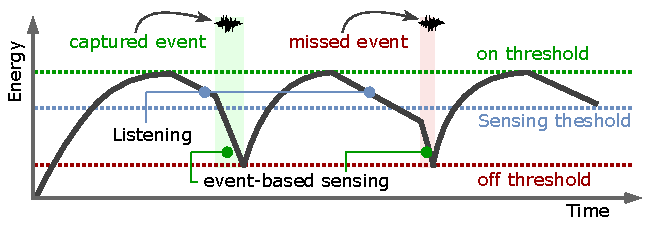
\includegraphics[width=\columnwidth]{figures/PowerCycleIntermittentSensor}
		\caption{When \sys does event-based sensing---staying in low power mode listening for an external event to happen---, its energy consumption profile has three distinct rates: zero when it is charging, a maximum when it is sensing, and an in-between energy consumption rate when it is listening. The third rate requires special attention when designing a \sys.}
		\label{fig:eventBasedSensing}
\end{subfigure}
		\caption{\fullsys energy profile for different sensing strategies}
		\label{fig:cisPwrCycle}
\end{figure} 
%
An intermittent sensor has a limited energy budget per power cycle. When it is tasked with a polling-based sensing activity, its energy consumption, generally, switches between two levels: zero when charging and a maximum when it activates its microcontroller for data acquisition and processing, (see Figure~\ref{fig:pollingBasedSensing})---we assume that the microcontroller is the dominant energy consumer module of a node. However, in event-based sensing, a node puts its microcontroller into low power mode and waits (or listen) for an external event to wake up the microcontroller. This is important to minimize the energy wasted on the listening and to maintain the required energy budget for sensing for the longest possible time (Figure~\ref{fig:eventBasedSensing}). The idle listening mode, which is important for successful sensing, complicates the design of the \sys.

\subsection{On-time}
%
\begin{figure}[t]
		\centering
		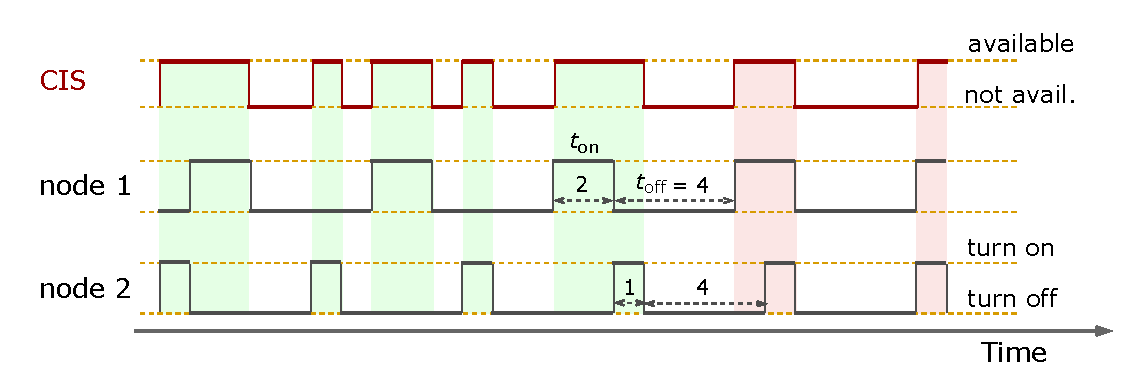
\includegraphics[width=\columnwidth]{figures/cisOntime}
		\caption{\fullsys's on-time is the projection of its intermittent nodes uptimes on the time axis. When the power cycles of the intermittent nodes are different their uptimes distribution approaches uniform distribution.}
		\label{fig:cisOntime}
\end{figure} 
%
The \sys's on-time is the projection of its underlying intermittent nodes' uptimes on the time axis. The \sys's on-time ranges from minimum (when all nodes on-times cluster together, see the red regions in Figure~\ref{fig:cisOntime}) to the maximum (when the overlapping between its nodes uptimes is zero or when the continuous time is reached). Two broad controlling strategies for minimizing nodes on-times clustering and maximizing \sys's time span can be imagined: 
\begin{enumerate}[label=\roman*.]%[wide, labelwidth=!, labelindent=0pt]
%
		\item \textit{Explicit on-time division strategy}: Recent advancements in timing intermittent operations enable intermittent nodes to measure their on and off times with the help of an external ultra-low-power timer~\cite{mayfly2017hester}. Similar breakthroughs in passive communication~\cite{marco} enable ultra-low-power message exchange between batteryless nodes. Intermittent nodes can use these recent advancements to apply time division multiplexing strategy to explicitly avoid nodes on-times clustering. For example, a node calculates its average on-time $\overline{t_{on}}$ and off-time $\overline{t_{off}}$ for $N$ power cycles. Then it measures the time difference between its power-up and the intended transmitting time $\Delta\,t$. Then it encodes these information $({\overline{t_{off}}, \overline{t_{on}}, \Delta\,t})$ in a message and broadcasts it. If a node receives this message it will have full information about the transmitting node power cycle. It can then alter its power cycle, relative to the transmitting nodes cycle, by either increasing (or decreasing) its power consumption to shorten (or lengthen) its on-time and shift its power cycle to a different time slot. This approach, obviously, assumes relatively stable nodes power cycles. 
%
\begin{figure}
		\centering
		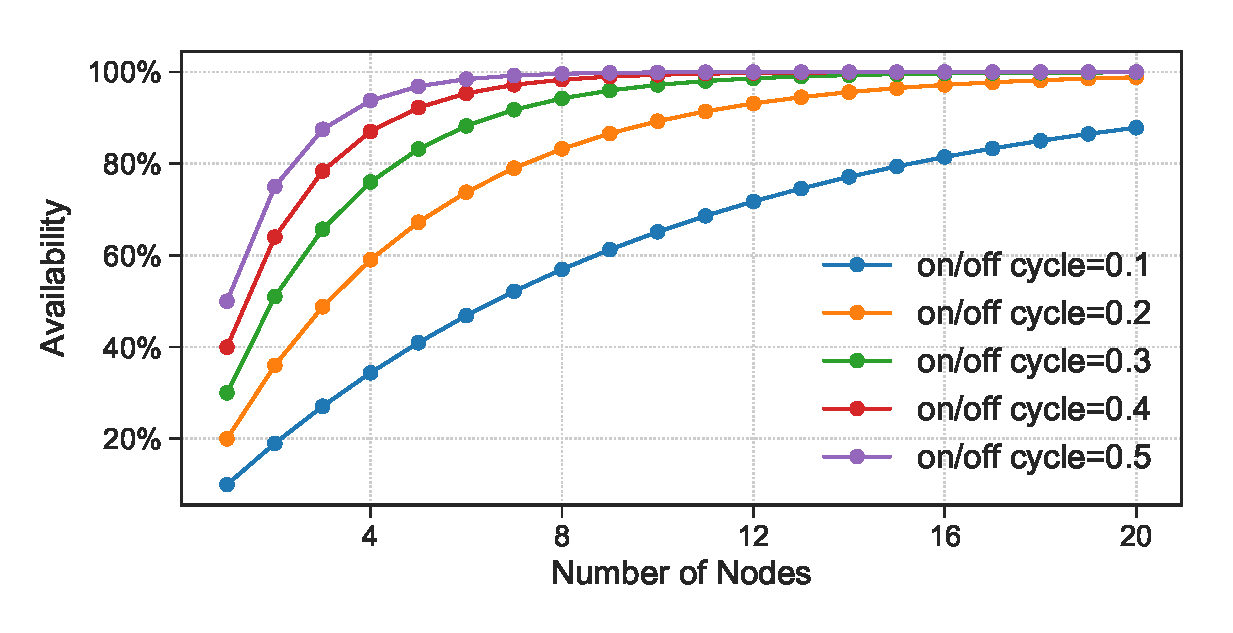
\includegraphics[width=\columnwidth]{figures/cisModel}
		\caption{\fullsys availability percentage for a different number of nodes and different duty cycles. The nodes are uniformly distributed and the \sys on-time evolves according to the equation~\ref{eq:cisModel} when new nodes are added.}
		\label{fig:cisModel}
\end{figure} 
%
		\item \textit{Implicit on-time division strategy}: With no information being exchanged between intermittent nodes, the best \sys can do is to uniformly distribute its node's on-times and maintaining this distribution over time. The key observation to uniformly distribute the nodes' on-times is to ensure that their power cycles are different. This can be achieved by forcing intermittent nodes to go into low-power-mode upon power-ups. The length of this mode is randomly chosen for each node. This will change the length of the nodes on-times and, consequently, alter their power cycles. Figure~\ref{fig:cisOntime} shows the scenario of two intermittent nodes with different power cycles. Node 1 has a power cycle of 6 units of time and an on/off cycle of $\frac{1}{3}$. Node 2 has a power cycle of 5 units of time and an on/off cycle of $\frac{1}{5}$. Following the time axis from the left, we can see that the position of the on-time of Node 2 is shifted by 1 unit of time after each power cycle of Node 2. This implies that the on-times of the two nodes are $\frac{1}{3}$ of the time cluster together and $\frac{2}{3}$ of the time they are apart. If we extend the previous scenario to three or more nodes then the on-time of the resulting \sys can be described with the following formula,
				
\begin{equation}
	t_{on}(N) = t_{on}(N-1) + \frac{t_{off}(N-1)}{t_{off}(N-1)+t_{off}(N-1)} \times t_{on}(1),
		\label{eq:cisModel}
\end{equation}
where $t_{on}(N)$ is the on-time of a \sys with $N$ intermittent nodes. Figure~\ref{fig:cisModel} shows the \sys availability percentage for different duty cycles and different number of intermittent nodes.
\end{enumerate}
There is a clear trade-off between the aforementioned methods. While the explicit control method provides fine control over the system distribution, the implicit method does not suffer from control messages exchange overhead. Although the implicit method is relatively simple to implement and explore, the explicit control method is not a far fetched idea considering the recent advancements in passive communication and intermittent timing. However, we opt to explore the implicit distribution control method as the hardware used to demonstrate the feasibility of passive light communication and ambient RF backscattering are not open source and re-making it is beyond the scope of this study.

\subsection{Power States}
A \sys can experience a wide range of ambient power intensity. For example, a solar-powered \sys may harvest no energy at night, modest energy from artificial light, and much more from direct sunlight.  Generally, we can identify four different \sys powering states: 
\begin{enumerate}
		\item \textit{Targeted energy conditions}---These are the energy conditions that the \sys designed for. In these energy conditions, the \sys should work intermittently and have sufficient power cycles randomness to uniformly distribute its intermittent nodes on-times and meet the desired availability percentage. In general, the targeted energy conditions should be near worst energy harvesting conditions to ensure that the system is properly functioning for the majority of the time.
		\item \textit{Under-targeted energy conditions}---Ultimately, the ambient energy is an uncontrollable power source, and it is not hard to imagine scenarios where a \sys will be underpowered or even comes to complete and long power down (for example, a solar \sys will come to a perpetual power down in the darkness). In general, for under-targeted energy conditions, the \sys behavior can be considered as undefined.
%
\begin{figure}
		\centering
		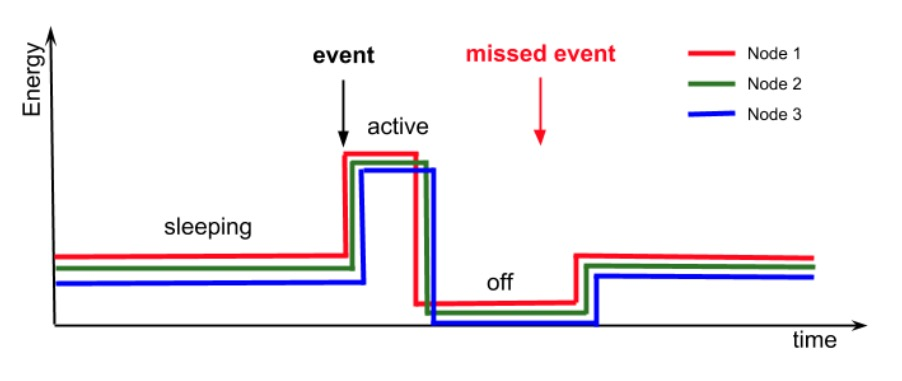
\includegraphics[width=\columnwidth]{figures/noRandomization}
		\caption{\todo{Placeholder} No randomization}
		\label{fig:noRand}
\end{figure} 
%
		\item \label{it:hibernating} \textit{Hibernating energy conditions}---when \sys is tasked with event-based sensing, and the energy conditions are relatively higher than the targeted conditions, then the harvested energy may compensate for the energy consumption of the low-power mode. Thus, the system loses its randomness feature, and all the nodes will react to the first external event and power down shortly after as the energy consumption of sensing and processing is much higher than the energy consumption of the low-power-mode idle listening. If the external events happened to be sporadic, then this is not a big issue. However, for a bursty type of events (i.e. a command of two or three words), this will prevent the \sys from meeting its goal: continuous sensing (Figure~\ref{fig:noRand}). 
		\item \label{it:continuous} \textit{Continuously powered}---Under direct mid-noon sun even a tiny solar panel can continuously power a sensor. In such conditions, the \sys will sense continuously without the need for randomization. Therefore, the job of a single node will be repeated $N$ times, and instead of sending a single message to a battery-powered or tethered sink---to push the data to the internet---$N$ identical messages will be sent which waste a lot of energy. 
				
\end{enumerate}
%
\begin{figure}
		\centering
		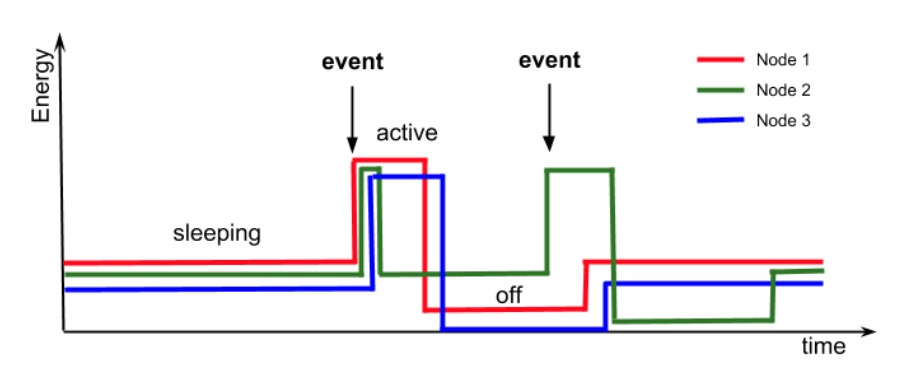
\includegraphics[width=\columnwidth]{figures/randomization}
		\caption{\todo{Placeholder} Randomization}
		\label{fig:rand}
\end{figure} 
%
\begin{figure}
		\centering
		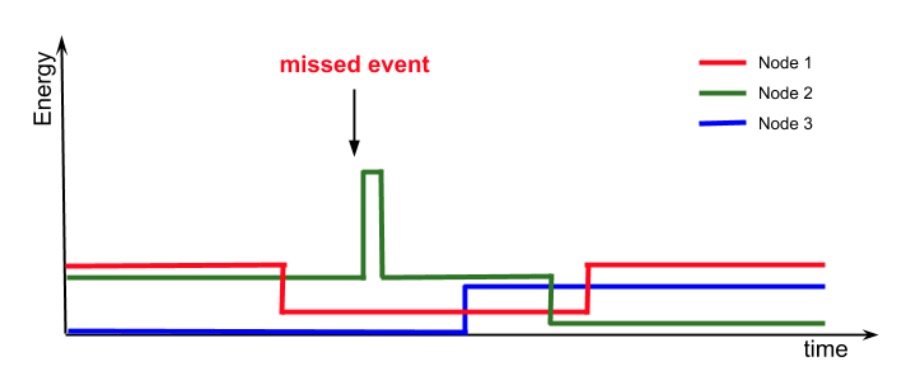
\includegraphics[width=\columnwidth]{figures/randomizationSideEffect}
		\caption{\todo{Placeholder} Randomization side effect}
		\label{fig:randSideEffect}
\end{figure} 
%
The problems mentioned in~(\ref{it:hibernating}) and (\ref{it:continuous}) can be mitigated by enforcing randomization on the response of the intermittent nodes (Figure~\ref{fig:rand}): when a node is wakened up by an external event it responds to that event with a certain probability. However, if the randomized response is enforced all the time, then the \sys will have a lower probability of catching events during the targeted energy conditions (Figure~\ref{fig:randSideEffect}). Therefore, the \sys has to distinguish between the targeted and above-targeted energy conditions and apply response randomization only during the above-targeted energy conditions. To do this, an intermittent node can measure the energy intensity using a dedicated ultra-low-power sensor or using the on-time duration as a metric to estimate the ambient energy intensity. A node energy buffer holds a certain maximum amount of energy, know during manufacturing. This energy powers the node for a certain amount of time $t_{nopwr}$ for a fixed load $l_{fix}$. $t_{nopwr}$ can be embedded in the intermittent node memory before deploying. When the node wants to measure the incoming power, it set its load to $l_{fix}$ and measure its on-time $t_{pwr}$. The time difference between $t_{pwr}$ and $t_{nopwr}$ can be used as a metric to estimate the incoming power and choose the response probability accordingly.

%For a large \sys system, choosing a fix response probability is an inefficient way of dealing with the over-powering problem. As the number of active intermittent nodes at a given time is a function of the total number of nodes and the power intensity at that time. Power intensity can be measure or inferred from the node on-time.   


%To meet a certain system availability, the system needs to be design for low energy conditions (i.e. artificial light).Depending on the ambient energy conditions, a \sys's power can vary significantly.  Generally, we can define four operational conditions that a \sys can experience.




